%!TEX root = ../dissertation.tex
\begin{savequote}[0.6\textwidth]
	\itshape In the beginning, there was nothing. \\
	\itshape And God said, Let there be light. \\
	\itshape And there was light. \\
	\itshape There was still nothing, \\
	\itshape but you could see it a lot better.
	\qauthor{---Woody Allen}
\end{savequote}

\chapter{GaudiMM}
\label{chap:04}


\Lettrine{There} is an implicit restriction in multiscale approaches due to their own design. They are based on a sequential series of steps, which are chained one after another to answer the initial question. Each step must be resolved separately, which can potentially become a bottleneck or even a blocking step if the results are not successfully obtained.

% Indirectly, methods that suffer from insufficient sampling capacity can only operate with subregions of the system under study, deliberately ignoring details outside that region.

Instead of forcing a sequential protocol around a complex molecular problem, an alternative approach could be devised. If the panoply of existing modeling methods could be recruited on demand to work simultaneously on the same study, all of them could contribute to solve the problem, multiplying their strengths and compensating their weaknesses. Building this feature set into a robust and flexible platform would be very desirable for drafting molecular hypotheses and sketching proofs of concept.

GaudiMM is here presented to become such a a platform. It takes the expresiveness and flexibility of Python to create a molecular design platform with unprecedented versatility. The rationale behind its concept can be summarized in three points:

\begin{enumerate}
	\item Its modular implementation allows to encapsulate separate methods in isolated entities that can work together through a well defined programmatic interface, which also allows fast development of new extensions.

	\item It makes a clear distintion between the three main stages of any optimization process (exploration, evaluation and selection), which suggests a flexible way of rationalizing molecular modeling problems.

	\item It does not require prior knowledge of the importance of the variables that affect the system thanks to its multi-objective optimization capabilities.
\end{enumerate}

As a result, solving a molecular modeling problem is only a matter of choosing the appropriate modules in terms of which variables should be explored (cartesian coordinates, chemical spaces...) and which properties should be measured (geometries, energies...). In some cases, some rigor can be sacrificed in honor of obtaining good enough results to start working with. In other cases, the combination of methods will work synergestically towards the design of a novel methodology.

Following sections will describe: (1) the algorithmic and (2) implementation details of the platform, (3) how different combinations of modules allow diverse molecular modeling tasks, and (4) how to analyze the proposed results.

%%%%%%%%%%%%%%%%%%%% Table No: 1 starts here %%%%%%%%%%%%%%%%%%%%


\begin{table}[hbtp]
	\caption{GaudiMM: technical datasheet}
	\footnotesize
	\newcolumntype{R}{>{\hsize=.25\hsize\raggedleft\arraybackslash}X}%
	\newcolumntype{L}{>{\hsize=.75\hsize\raggedright\arraybackslash}X}%
	\newcommand{\tableheading}[1]{\multicolumn{2}{c}{\textsc{#1}}}
	\begin{tabularx}{\textwidth}{RL}
		\toprule
		%row no:1
		\tableheading{GaudiMM} \\
		\toprule
		%row no:2
		\textit{Description} & A modular optimization platform for molecular design \\
		\midrule
		%row no:3
		\textit{Requirements} & Python, UCSF Chimera, OpenMM, IMP, DSX, ProDy... \\
		\midrule
		%row no:4
		\textit{License} & Apache 2 \\
		\midrule
		%row no:5
		\textit{Download} & \href{https://github.com/insilichem/gaudi}{github.com/insilichem/gaudi} \\
		\midrule
		%row no:6
		\textit{Documentation} & \href{https://gaudi.readthedocs.io}{gaudi.readthedocs.io} \\
		\midrule
		%row no:7
		\textit{Citation} & J. Comput. Chem. 2017, 38, pp 2118–2126. DOI: 10.1002/jcc.24847 \\
		\bottomrule

	\end{tabularx}
\end{table}


%%%%%%%%%%%%%%%%%%%% Table No: 1 ends here %%%%%%%%%%%%%%%%%%%%

\section[Algorithmic details]{Algorithmic details: \\ multiobjective optimization \& NSGA-II}

GaudiMM is built on top of a multiobjective genetic algorithm (MOGA), NSGA-II, developed by K. Deb.\cite{nsgaii} It has been thoroughly tested and benchmarked in well-characterized multi-objective problems and is considered a prototypical MOGA.

As other optimization methods, this algorithm can be described in three main stages (exploration, evaluation and selection) that are executed iteratively until an exit condition is met (usually, convergence or maximum steps). Generating new candidate solutions or individuals is considered within the \textit{exploration} stage, and can be achieved by random attribute assignation or combining previously existing individuals. In the \textit{evaluation} stage, the candidates are assessed with different functions or objectives, each returning a scalar that represents a fitness score for that objective. Finally, the selection stage collects all the individuals and compares their vectorial scores to select the best individuals according to the Pareto dominance criterion (see \autoref{chap:02}).

In more detail, NSGA-II starts with the generation of a random set of potential solutions (\textit{individuals}) which comprise the so-called \textit{initial population}. This first set of individuals is then evaluated with one or more \textit{objectives} and each individual is assigned a \textit{fitness} score vector, the elements of which are the result of those cost functions. At this point, a small subset of the population is submitted to a round of random modification of parameters (\textit{mutation}) or exchanging some of their attributes (\textit{recombination}), and are then assessed by the same cost functions. Being random, the results of these variations can be better or worse than their preceding counterparts (parents). Finally, both the offspring and the parental generation ($ \mu $ +$ \lambda $ strategy) compete in the selection tournament, which will rule which ones will replace the initial population. After a number of iterations, the initial population will have evolved and, eventually, will end up providing reasonable solutions to the problem that represent a compromise between the analyzed variables (see fig. \ref{fig:nsga}).

\begin{figure} % FIXME!
	\vspace*{-1cm}
	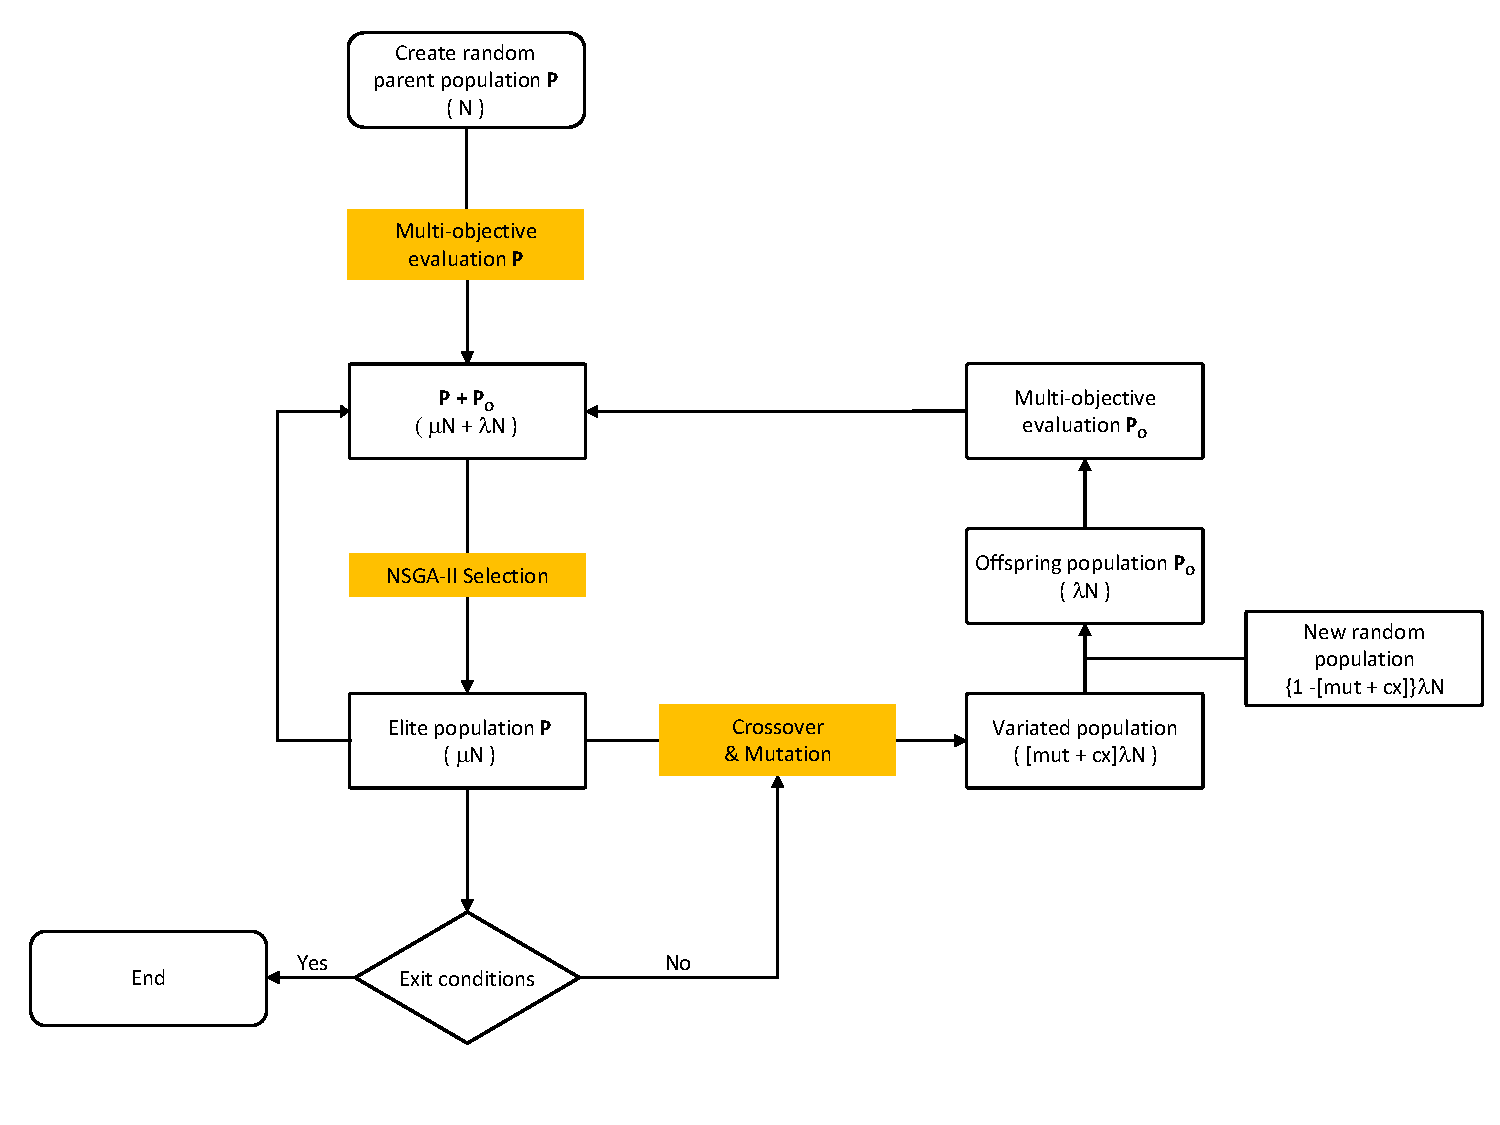
\includegraphics[width=0.9\textheight,angle=90]{./figures/04/nsga.pdf}
	\cprotect\caption[NSGA-II algorithm]{Flowchart of the modular NSGA-II multi-objective genetic algorithm (MOGA) implemented in GaudiMM. $ N $ is the number of individuals in the initial population $P$. Values $\lambda$ and $\mu$ are related to the number of children produced at each generation and the number of individuals selected for the next generation, respectively. Together they control the offspring population size, $ P_{0} $. Constants $ mut $ and $ cx $ are the probabilities associated to mutation and crossover.}
	\label{fig:nsga}
\end{figure}


\section{Implementation}

The underlying algorithm is very present in how GaudiMM has been implemented and how it is used. Learning to model with GaudiMM means having a clear understanding on the different stages involved in the algorithm, specially exploration and evaluation.

\subsection{Of individuals and genes: the exploration stage}
% \addcontentsline{toc}{subsection}{Of individuals and genes: the exploration stage}
The initial step of all the iterations in the algorithm is the exploration, which is responsible for the generation of new candidate solutions. A candidate solution is defined by a list of attributes, each representing the state of a molecular property. Generating new solutions simply involves changing the value of one or more attributes in that list.

Since GaudiMM is based on a genetic algorithm, the implementation follows the same biologicist terminology. In GaudiMM any candidate solution is encoded in a special object called \texttt{Individual}. All \texttt{Individual} objects in the simulation are defined by the same high-level attributes, which are called \textit{genes}. In the same fashion, the state of each gene is defined by its \textit{allele} attribute. Depending on the gene, the allele can be a list of numbers, a path to a file, a matrix$ \ldots $

For example, a typical optimization problem is finding the dihedral torsion that gives the minimum energy in the ethane molecule. The \texttt{Individuals} featured in this example would only need exploring a single variable, the torsion angle of the C-C bond, with values ranging from 0 to 360$^\circ$. In GaudiMM-speak, the gene would be the bond \textit{rotator} and the allele the different angles.

The key part of genetic algorithms is the implementation of variation operators as part of the exploration stage. Instead of merely trusting randomness, existing solutions are combined in hopes of obtaining a better child solution. These two operations are called \textit{mutation} and \textit{crossover} or mating, mimicking what happens in the cell nucleus at the chromosomic level.


\begin{figure}[H] % FIXME!
	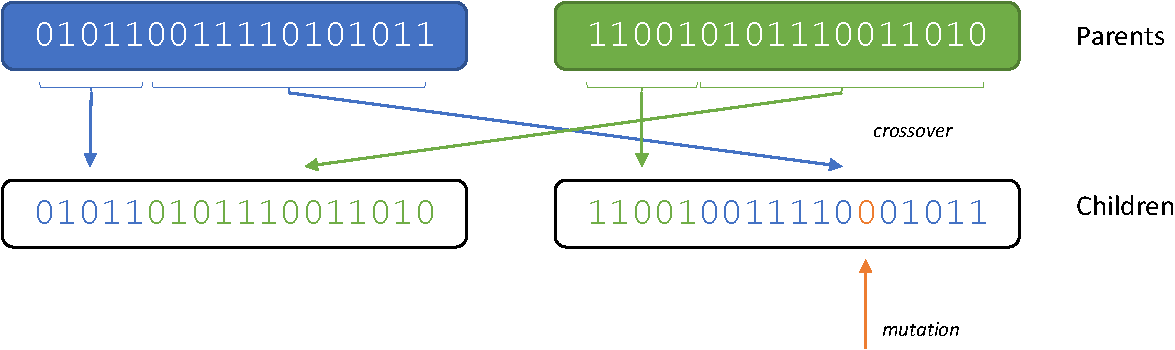
\includegraphics[width=\textwidth]{./figures/04/ga-crossover-mut-crop.pdf}
	\caption[Mutation and crossover]{Mutation and crossover operations introduce variability in the parental population.}
	\label{fig:cxmut}
\end{figure}

Taking all these requirements into account, genes in GaudiMM are programmatically defined by four functions (\texttt{express}, \texttt{unexpress}, \texttt{mutate} and \texttt{mate}) and an attribute (\texttt{allele}). Additional methods and attributes can be defined to support these required elements, if needed. Since each gene is a clearly separate entity, the \textit{Individual} object can feature more than one gene, and one gene can be present more than once with different parameters.

This adds an unprecedented versatility when configuring a GaudiMM calculation: the user can decide which molecular features must be explored for every case. For conformational searches it might be enough with the \texttt{Torsion} gene, but for protein-ligand docking the \texttt{Search} gene will be required too. Additionally, if the built-in genes do not fulfill the requirements of the simulation, new ones can be written and added to GaudiMM thanks to is modular architecture and well-defined programmatic interface.

This is, genes are more than simple \textit{allele} attribute holders: they are high-level abstractions of operators that can make reversible changes in a molecule based on the value of its allele. Like in Biology, changes in the allele are only visible if the corresponding gene is being \textit{expressed}. In those terms, GaudiMM genes encompass both the allele and the expression mechanism. In the previous example, when the allele changes the torsion gene needs to update the coordinates of the atoms affected by the dihedral rotation, and only those. To make changes consistent, it might also need to \textit{unexpress} or undo those changes to the original state. These changes can happen in the topology or coordinates of an associated molecule.

\subsubsection{Topology modifiers}
% \addcontentsline{toc}{subsubsection}{Topology modifiers}
Genes that fall in this category perform modifications on the atoms that conform the molecular structure and/or their connectivity. For example, they could increase the length of a ligand linker, change the metal element of a metallic cofactor or mutate some residues in a peptide sequence.

\begin{itemize}
	\item \textsc{Molecule}. It is the main gene, as it will be used to load molecular structures from files (\texttt{PDB}, \texttt{Mol2}, \texttt{XYZ} or any other input format supported by UCSF Chimera). All other genes depend on the initial topology and coordinates provided by one or more Molecule genes. In addition to loading files, the \texttt{path} parameter supports loading from a directory, whose contents determine the final behavior:
	\begin{itemize}
		\item If the directory contains molecule files, the allele will be set to one of them randomly for each individual. This allows GaudiMM to deal test a library of compounds against certain criteria; i.e. virtual screening.
		\item If the directory contains subdirectories which, in turn, contain molecules files, the gene will sort those subdirectories by name and then pick one molecule from each, in that order. The chosen molecules will constitute the allele and will be chained linearly as specified in the accompanying meta file, which lists the serial number of the potential donor and acceptor atoms.
	\end{itemize}
	\item \textsc{Mutamers}. Given a residue position in a protein structure, it can replace its sidechain to any other natural amino acid specified in the configuration. Useful to study site mutations.
\end{itemize}

\subsubsection{Coordinates modifiers}
% \addcontentsline{toc}{subsubsection}{Coordinates modifiers}
Genes that fall in this category only alter the positions of the atoms involved in a molecular structure. They can modify the full structure, like a rigid translation or rotation of the molecule, or only a part, like the sidechain orientation of a protein residue.

\begin{itemize}
	\item \textsc{Torsion}. It helps explore small molecules flexibility by performing bond rotations in the selected \texttt{Molecule} objects, if they exhibit free bond rotations.

	\item \textsc{Search}. It performs rigid transformations on \texttt{Molecules} (translation and rotation). A radius parameter can be set to limit the search sphere range. If the radius is zero, the molecule will not be translated but can freely rotate around the anchor atom, which is useful for covalent bond emulation.

	\item \textsc{Rotamers}. It allows to explore side-chain conformations in protein residues by applying Dunbrack's\cite{dunbrack1993backbone} or Dynameomics\cite{scouras2011dynameomics} rotamer libraries.

	\item \textsc{NormalModes}. Given a \texttt{Molecule} object, it calculates normal modes with elastic network methods and applies the resulting collective motions as possible variants of the initial coordinates set.

	\item \textsc{Trajectory}. Given a molecular dynamics trajectory file, it can retrieve random frames and apply the resulting coordinates to any Molecule object.
\end{itemize}


\begin{table}[hbtp]
	\caption[List of genes implemented in GaudiMM]{List of genes implemented in GaudiMM.}
	\label{table:gaudi-genes}
\footnotesize
\newcolumntype{L}{>{\hsize=.25\hsize\raggedright\arraybackslash}X}%
\newcolumntype{M}{>{\hsize=.5\hsize\raggedright\arraybackslash}X}%
\newcolumntype{R}{>{\hsize=.25\hsize\raggedright\arraybackslash}X}%
\begin{tabularx}{\textwidth}{LMR}
%row no:2
\toprule
\textsc{Name} & \textsc{Description} & \textsc{Depends on} \\
\toprule
%row no:3
 Molecule & Load and build structures & UCSF Chimera \\
\hhline{~~~}
%row no:4
 Rotamers & Explore side chain flexibility & UCSF Chimera \\
\hhline{~~~}
%row no:5
 Mutamers & Explore mutation of residues & UCSF Chimera \\
\hhline{~~~}
%row no:6
 NormalModes & Explore collective motions & ProDy\cite{prody} \\
\hhline{~~~}
%row no:7
 Search & Translation and rotation of Molecules & UCSF Chimera \\
\hhline{~~~}
%row no:8
 Torsion & Dihedral rotation of bonds & UCSF Chimera \\
\hhline{~~~}
%row no:9
 Trajectory & Load frames from MD trajectories & MDTraj\cite{mdtraj} \\
\bottomrule
\end{tabularx}
\end{table}


%%%%%%%%%%%%%%%%%%%% Table No: 2 ends here %%%%%%%%%%%%%%%%%%%%



\subsection{Of environments and objectives: the evaluation stage}
% \addcontentsline{toc}{subsection}{Of environments and objectives: the evaluation stage}
After generating candidate solutions, these must be evaluated with the optimization criteria. In genetic algorithms, this is usually called assessing the fitness of the individuals: fitter individuals are more qualified to survive in the environment.

Mimicking these concepts, the GaudiMM implementation creates an \texttt{Environment} object that list the optimization criteria, each represented by an \texttt{Objective} entity. Objectives are also independent units that can be instantiated multiple times in the same \texttt{Environment}, but the defined interface is simpler that in genes: a \textit{weight} attribute defines the optimization type (maximization or minimization), and a function named \texttt{evaluate} that takes an \texttt{Individual} object and returns a numerical value as result. What the \texttt{evaluate} function does behind the scenes does not actually matters as long as a number is produced: calculate a distance between two atoms, retrieve a parameter from a database, compute the potential energy with an external MM library$ \ldots $

As a result, GaudiMM ships with a rather diverse set of objectives, combining 3\textsuperscript{rd} party packages and custom developments in the same distribution. Together they cover all kinds of energetic, geometric and spatial measurements, allowing to use different levels of theory at the same time in a seamless workflow. Any geometric or energetic parameters that could describe a molecular system can be used as objectives to drive the GA exploration. This allows us to turn the tables on routine protocols based on computing energetic optimizations and then analyzing the results in hopes of finding a suitable model that fits the intended restraints; i.e. those same analysis tools can guide the optimization process from the beginning.

\subsubsection{Geometry measurement}
% \addcontentsline{toc}{subsubsection}{Geometry measurement}
\begin{itemize}
	\item \textsc{Angle}. Given three atoms, this objective calculates the angle between those. By minimizing the difference between the measured angle and the target one, the final angle can be optimized. It will calculate the dihedral if four atoms are specified.

	\item \textsc{Distance}. If two atoms are provided, this objective calculates the distance between. By minimizing the difference against a target value, the structure can be optimized to fulfill that requirement. It also supports calculating distances to groups of atoms by taking the centroid of the group.

	\item \textsc{Inertia}. This objective calculates the inertia tensors of two structures and returns the sine of the smallest angle formed between any of the possible pairings. It can be useful to align ligands along the major axis of a protein.


\end{itemize}\subsubsection{Spatial measurement}
% \addcontentsline{toc}{subsubsection}{Spatial measurement}
\begin{itemize}
	\item \textsc{Solvation}. Solvent-Accessible Surface Area (SASA) and Solvent-Excluded Surface Area (SESA) are two common techniques to describe the solvation of a structure. It can be used to optimize structures in terms of exposure of inside pockets or their folding. By maximizing SASA or SESA, the structure will tend to open up; by minimizing those values, the trend will be towards a more compact conformation.

	\item \textsc{Volume}. This objective calculates the volume occupied by a structure. It does so by computing the solvent-exposed surface of the structure, which is then considered as a polyhedron of thousands of triangular faces.


\end{itemize}\subsubsection{Energy calculation}
% \addcontentsline{toc}{subsubsection}{Energy calculation}
\begin{itemize}
	\item \textsc{DSX}. DrugScoreX is a knowledge-based docking scoring function developed by Neudert $\&$  Klebe.\cite{neudert2011dsx} It is specially designed to compute interaction energies between protein structures and small compounds. This objective is a Python wrapper around the DSX executables and input files.

	\item \textsc{Energy}. This objective allows to calculate the potential energy of a structure with the Molecular Mechanics force fields implemented in OpenMM. Parameters must be provided for custom residues.

	\item \textsc{LigScore}. Another docking scoring function developed by Sali\cite{krammer2005ligscore} which allows to obtain protein-ligand interaction energies. While the parent project, IMP,\cite{russel2012putting} is a C++ project with Python bindings, the LigScore function is only exposed through an executable. This objective can call that binary and parse the resulting energies from the output.

	\item \textsc{Vina}. AutoDock Vina\cite{trott2010autodock} is a popular open-source package to perform protein-ligand docking. This objective calls the Vina executable in score-only mode to calculate the interaction energies between a protein and a ligand.

	\item \textsc{GOLD}. This commercial software suite is one the most used solutions to calculate accurate docking poses. With this objective, all the scoring functions exposed in GOLD\cite{gold} can be used as guiding evaluators in GaudiMM: PLP, GoldScore, ChemScore$ \ldots $  License is needed for this to work.

	\item \textsc{NWChem}. This objective provides a way to run quantum mechanics calculations in this popular open-source software suite.\cite{nwchem} Provided a template input-file, this objective will insert the appropriate coordinates, charge and multiplicity. While all methods implemented in NWChem are potentially usable, only semi-empirical ones are recommended in terms of speed; specially for large structures.


\end{itemize}\subsubsection{High-level chemical descriptors}
% \addcontentsline{toc}{subsubsection}{High-level chemical descriptors}
\begin{itemize}
	\item \textsc{Contacts}. This objective can calculate two type of distance-based energy descriptors. When the \textit{hydrophobic} mode is chosen, this objective will maximize potentially attracting interactions between close enough atoms by applying a Lennard-Jones-like scoring function. If the \textit{clashes} mode is chosen, it will minimize the steric hindrance of the structure by minimizing the volumetric overlap of the Van der Waals spheres of atoms that are too close.

	\item \textsc{HBonds}. This objective uses geometrical criteria to calculate the number of hydrogen bonds between potential donors and acceptors.

	\item \textsc{Coordination}. By applying a type of computer vision algorithm called Point Set Registration, this objective can identify potential coordination geometries around a metal center. It returns the RMSD similarity between the first coordination sphere and the ideal polyhedron: the lower the value, the better the geometry.
\end{itemize}


\begin{table}[hbtp]
	\caption[List of objectives implemented in GaudiMM]{List of objectives implemented in GaudiMM.}
	\label{table:gaudi-objectives}
\footnotesize
\newcolumntype{L}{>{\hsize=.15\hsize\raggedright\arraybackslash}X}%
\newcolumntype{M}{>{\hsize=.65\hsize\raggedright\arraybackslash}X}%
\newcolumntype{R}{>{\hsize=.20\hsize\raggedright\arraybackslash}X}%
\begin{tabularx}{\textwidth}{LMR}
\toprule
\textsc{Name} & \textsc{Description} & \textsc{Depends on} \\
\toprule
%row no:3
 Angle & Optimize angle of three atoms, or dihedral of four atoms & UCSF Chimera \\
\hhline{~~~}
%row no:4
 Contacts & Minimize steric clashes, maximize hydrophobic interactions & UCSF Chimera \\
\hhline{~~~}
%row no:5
 Coordination & Optimize coordination geometry of metal center & In-house\cite{gaudimetals} \\
\hhline{~~~}
%row no:6
 Distance & Optimize distance between two or more atoms & UCSF Chimera \\
\hhline{~~~}
%row no:7
 DSX & Docking scoring function  & DrugScoreX\cite{neudert2011dsx} \\
\hhline{~~~}
%row no:8
 Energy & Minimize molecular mechanics potential energy & OpenMM\cite{openmm} \\
\hhline{~~~}
%row no:9
 HBonds & Detect hydrogen bonds  & UCSF Chimera \\
\hhline{~~~}
%row no:10
 Inertia & Align axes of inertia of two or more molecules & In-house \\
\hhline{~~~}
%row no:11
 LigScore & Docking scoring function & IMP\cite{krammer2005ligscore} \\
\hhline{~~~}
%row no:12
 NWChem & Launch NWChem QM calculations & NWChem\cite{nwchem} \\
\hhline{~~~}
%row no:13
 Solvation & Measure solvent accessible solvent area & UCSF Chimera \\
\hhline{~~~}
%row no:14
 Volume & Measure volume occupied by molecule & UCSF Chimera \\
\bottomrule

\end{tabularx}
 \end{table}


%%%%%%%%%%%%%%%%%%%% Table No: 3 ends here %%%%%%%%%%%%%%%%%%%%



\subsection{Of tournaments and trade-offs: the selection stage}
% \addcontentsline{toc}{subsection}{Of tournaments and trade-offs: the selection stage}
Once the \texttt{Individuals} have been assigned a fitness score, these values must be compared to assess how good of a solution they make. In multi-objective optimization problems there is no \textit{best} solution in usual terms. Instead, a set of trade-offs between the involved (and usually conflicting) variables is required. NSGA-II solves this by following the Pareto optimality criterion explained in \autoref{chap:02}, which will iteratively enrich the Pareto optimal set with the \textit{best} candidates of the population. However, when more variables (objectives) are added to the optimization, the Pareto front grows in dimensionality and enriching the Pareto optimal set can get difficult. Deb et al do not recommend more than three objectives for NSGA-II, but several extensions to the algorithm are available (MONSGA-II, NSGA-III) exist to improve this situation. Higher dimensionality will also involve a larger number of possible solutions (even when Pareto-optimality is reached).

To ensure a rich Pareto front in constructed, NSGA-II includes a crowding parameter, and GaudiMM provides structural similarity comparisons when scores are very close to each other, resulting in a good compromise between diversity and number of solutions proposed.

\subsection{The code behind: Python as glue}

GaudiMM started by hooking \texttt{deap}\cite{fortin2012deap} evolutionary algorithms into UCSF Chimera. Using Python as the main language allowed to design a modular architecture that conceptually emphasizes the different stages of optimization, while focusing on the reutilization and addition of existing codebases. It is difficult to think of a different language that could have provided a working proof-of-concept in that little time.

All the code is object-oriented and features a well-documented programmatic interface, alleviating the process of writing new genes and objectives. The educational value of this technical decision was not obvious until degree and master students began to collaborate in the project as part of their final dissertation (see \autoref[appendix]{chap:appendix-b}).

After years of development, UCSF Chimera is still the main library behind the scenes. In fact, to our knowledge, GaudiMM is one of the few projects that relies on it for calculation purposes and not strictly for visualization. This interactive 3D viewer offers lots of analysis tools and robust molecular abstractions that allowed us to implement most of GaudiMM genes and objectives in few lines of code. However, everything has a price and UCSF Chimera was not designed to be used as a library in other projects; instead it expects external projects to be executed within UCSF Chimera interface. To overcome this limitation, a separate package named PyChimera was developed. With PyChimera, other Python libraries can be used together with UCSF Chimera, which allowed to intertwin other projects in GaudiMM. That way, MM energies can be computed with OpenMM, Normal Modes Analysis calculated with ProDy, and more (see tables \ref{table:gaudi-genes} and \ref{table:gaudi-objectives}). Further examples of integration are given in \autoref{chap:05}, where PyChimera has been instrumental in the development and distribution of new graphical interfaces.

\section{Usage: from recipes to molecular modeling tasks}

GaudiMM does not make any assumptions on the molecular modeling task to be performed. Setting up a calculation it is a matter of choosing the appropriate genes and objectives (see tables \ref{table:gaudi-genes} and \ref{table:gaudi-objectives}). Like ordering off a menu, each combination of those can be considered a \textit{recipe}. Since each gene and objective is a separate module that can be instantiated as many times as needed, this confers lots of flexibility.

All calculations normally start by configuring one or more \texttt{Molecule} genes to load the structures under study. On top of the \texttt{Molecule} genes, the user can choose additional genes to introduce certain types of variability, like the internal flexibility of a small compound (\texttt{Torsion} gene) or 3D spatial exploration (\texttt{Search} gene). Additional genes can target one or more \texttt{Molecule} genes, either partially or globally.

The set of genes will simply generate different variants of the starting model, which can potentially include non-feasible structures. As a result, after choosing which genes to apply, the user must decide which variables will guide the optimization of the structure by choosing one or more objectives. For example, it is common to request a \texttt{Contacts} gene to minimize the steric clashes that can arise from moving a small molecule around a bigger one.  If more requirements are needed, like maximizing the number of hydrogen bonds, the corresponding objectives can be added too.

It must be remembered that the objectives simply assign a score to a candidate solution. It is up to the selection step to favor the promotion of candidates that satisfy the optimization criteria (i.e., low number of clashes with good hydrogen bonds) and discard those that do not. As an example, a trivial molecular modeling task will be explained.

\subsection{Tutorial: Obtaining a cyclic alkane}

Building a cyclic alkane seems like a trivial task, but depending on the number of bonds involved, it can soon become a tedious process. With GaudiMM, it can be done in a single calculation: only two genes and two objectives are needed. The hypothesis is that there exists a set of dihedral torsions that can connect the ends of a linear decane without steric clashes.

First, a starting 3D structure is needed. For practical purposes, a linear decane can be built directly with UCSF Chimera by issuing the command \texttt{`open smiles:CCCCCCCCCC`} and saved as a Mol2 file with \texttt{`write decane.mol2`}. This file can be loaded in GaudiMM with a \texttt{Molecule} gene by setting its location as the value of the argument \texttt{path}.

The second gene is \texttt{Torsion}, which will detect rotatable bonds in the decane and apply the rotations instructed. However, the \texttt{Torsion} gene does not know nor care about steric clashes or minimum distances needed for a covalent bond. It will simply generate arbitrary sets of rotations.

Detecting one that can provide a structure compatible with a cyclodecane is responsibility of the evaluation stage. For example, to discard candidates with bad steric clashes, these should be minimized with the \texttt{Contacts} objective. In order to locate a structure compatible with a cyclodecane, a second objective is needed: a \texttt{Distance} minimization between the end carbon atoms of the decane. By setting the target distance as 1.5 Å, the linear decane will be forced to anneal itself.

This configuration is enough to run a simple multi-objetive optimization process. Since the \texttt{Contacts} objective only analyzes the volumetric overlap of the van der Waals spheres of the atoms and UCSF Chimera provides a basic library of van der Waals radii for all elements, no additional parameterization is needed. After running the program over this input file (see fig. \ref{fig:gaudimm-input-file}), GaudiMM will generate solutions compatible with the satisfaction of both criteria, which can be assessed with the accompanying graphical interface (see \autoref[section]{section:gaudimm-results}).

\begin{figure}[hbtp]
	\lstinputlisting[basicstyle=\small\ttfamily,language=Python]{./figures/04/input.yaml}
	\caption[GaudiMM input example]{Minimal GaudiMM input file for the optimization of linear decane into a cyclodecane.}
	\label{fig:gaudimm-input-file}
\end{figure}

However, after the first attempt, the user might realize that some of the results are indeed decane conformations whose ends are 1.5 Å apart, but not in the expected orientation. In other words, they do not respect the sp\textsuperscript{3} tetrahedral geometry. To fix it, an additional \texttt{Angle} objective set to match 109.5$^\circ$ between the end atoms and one of their neighbours would suffice. The final recipe can be consulted in table \ref{table:cyclodecane}.

\begin{table}[hbtp]
	\caption{Final recipe for the cyclodecane example}
	\label{table:cyclodecane}
	\footnotesize
	\newcolumntype{R}{>{\hsize=.25\hsize\raggedleft\arraybackslash}X}%
	\newcolumntype{L}{>{\hsize=.75\hsize\raggedright\arraybackslash}X}%
	\newcommand{\tableheading}[1]{\multicolumn{2}{c}{\textsc{#1}}}
	\begin{tabularx}{\textwidth}{RL}
		\toprule
		%row no:1
		\tableheading{Genes}\\
		\toprule
		%row no:2
		\texttt{Molecule} & Load the starting linear decane structure \\
		\midrule
		%row no:3
		\texttt{Torsion} & Explore rotations in rotatable bonds \\
		\toprule
		%row no:4
		\tableheading{Objectives}\\
		\toprule
		%row no:5
		\texttt{Contacts} & Minimize steric clashes \\
		\midrule
		%row no:6
		\texttt{Distance} & Bring terminal carbon atoms within 1.5 Å \\
		\midrule
		%row no:7
		\texttt{Angle} & Force terminal carbon atoms to match a $109.5^\circ$ angle \\
		\bottomrule

	\end{tabularx}
\end{table}

Albeit useless, this toy example illustrates the flexibility of the paradigm proposed in GaudiMM. For more practical use cases, please refer to models detailed in \autoref{chap:06}.

\section{Analyzing the results of multi-objective optimization}
\label{section:gaudimm-results}
In multi-objective optimization (see \autoref[section]{section:multiobjective}), ultimately choosing which solution is the \textit{best} is up to the decision maker: the researcher. Some strategies to make that decision involve reducing the fitness vector to a scalar using an adequate function. However, since that function is usually not characterized in tentative molecular modeling tasks, a UCSF Chimera extension has been developed GaudiView along GaudiMM to aid in that decision in a more interactive manner.

GaudiView will list the proposed solutions along with the fitness of each objective in spreadsheet-like dialog. Upon clicking each entry, the UCSF Chimera canvas will load and render a 3D interactive depiction of the structure. The table can be sorted by columns and filtered by threshold criteria, which can reduce the complex surface of the Pareto front to the \textit{interesting parts} (according to the decision maker) dynamically. Since the renderization of molecular structures is delayed until the corresponding rows are selected, the interface can show thousands of results with low memory usage. Integrative analysis can be performed on the flow with other tools included in UCSF Chimera thanks to the built-in command line widget, which is executed on each selection change event. \autoref[Appendix]{appendix:more-tangram} contains more details on this tool.


\begin{figure}[H]
	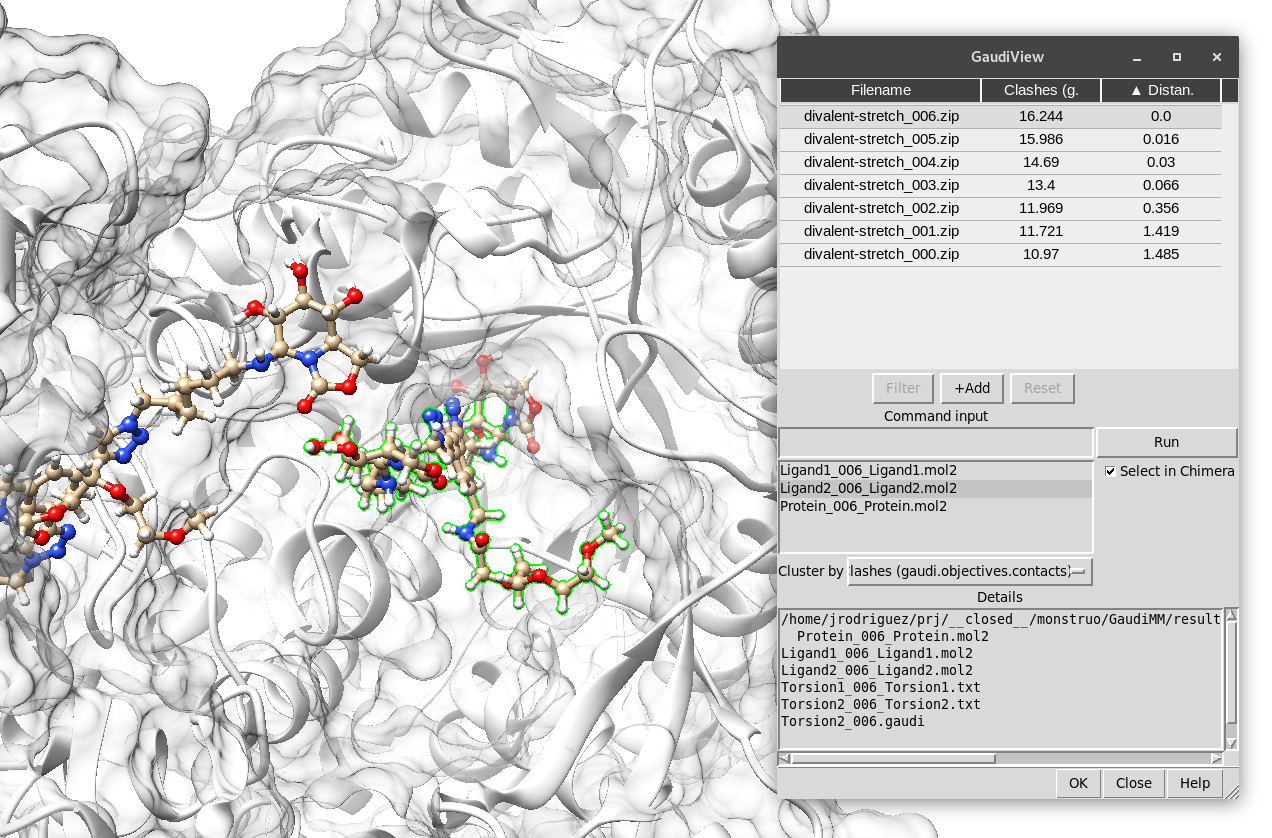
\includegraphics[width=\textwidth]{./figures/04/gaudiview.png}
	\caption[GaudiView]{Analysis of a GaudiMM dual docking calculation with GaudiView. Each row of the table represents one candidate solution that will be depicted in the 3D canvas upon selection.}
	\label{fig:gaudiview}
\end{figure}


\section{Conclusions $\&$  Further work}
% \addcontentsline{toc}{section}{Conclusions $\&$  Further work}

The development of GaudiMM was motivated by the need of applying simple descriptors in complex biomolecular systems featuring residues beyond the natural amino acids: metallic cofactors, oligosugar-derivatives and partially characterized organic molecules. The main idea was to at least have \textit{some} results around a hard-to-model structure, instead of saying that it could not be done. Even with low accuracy methods, GaudiMM soon started to prove that the approach is good enough to provide starting points valid for further refinement and processing with more accurate methods; in other words, GaudiMM is a good entry point for multiscale protocols. This and other examples of its potential applications, including how it has been used in real cases of research, will be detailed in \autoref{chap:06}.

These observations have made clear that GaudiMM provides a mental framework suitable for implementing proof-of-concept multiscale protocols and explaining basic concepts of molecular modeling to newcomers in the field.

That said, there is room for improvement in the performance area. Genetic algorithms are easily parallelizable by design, but depending on UCSF Chimera for most of the functions means that communication across processes could be expensive in terms of memory usage and synchronization overhead. Since the calculations rarely involve more than a few hours, the focus shifted towards the implementation of new modules rather than optimizing the speed of the new ones. However, it is one of the main milestones of the GaudiMM v2.0 roadmap.
